\chapter{Real-valued Optimization Algorithms}
\label{chapter:algos}

Overview of real-valued optimization

\section{Covariance Matrix Adaptation Evolution Strategy}

Describe history of \textit{Evolutionary Strategies} (ES).

The simplest algorithm is (1+1)-ES.

Here we describe the (1+1)-ES with one-fifth success rule with independent restarts.

The pseudo code of (1+1)-ES is given in Algorithm~\ref{algo:1+1ES}.

Covariance Matrix Adaptation Evolution Strategy (CMA-ES) is an extended version fo CSA-ES with de-randomized adaptation of covariance matrix.

Describe the underlying covariance matrix model.

Describe how to update \textit{mean}.

Describe how to update \textit{covariance matrix}.

Describe \textit{step-size} control.



\begin{algorithm}%[t!]
\caption{(1+1)-ES with 1/5 success-rule}\label{algo:1+1ES}

$\boldsymbol{X}_{n}$: solution of the $n^{th}$ iteration, $\sigma_n$: step size of the $n^{th}$ iteration, \\
$N(\boldsymbol{0}, \boldsymbol{I})$: multivariant normal distribution with mean vector $\boldsymbol{0}$ \\ 
and identical covariance matrix $\boldsymbol{I}$.

\BlankLine
\SetKwInOut{Input}{input} \SetKwInOut{Output}{output}
\Input{ $f$: evaluation function }
\Output{ $X_{n+1}$: best solution }

\BlankLine
Initialize $\boldsymbol{X}_0, \sigma_0$ \\
\While{ termination criterion not met } {

    $\widetilde{\boldsymbol{X}}_n = \boldsymbol{X}_n + \sigma_n N(\boldsymbol{0}, \boldsymbol{I})$  \\

    \eIf{ $f(\widetilde{\boldsymbol{X}}_n) \leq f(\boldsymbol{X}_n) $}{
        $\boldsymbol{X}_{n+1} = \widetilde{\boldsymbol{X}}_n$ \\
        $\sigma_{n+1} = 1.5 \sigma_n$
    }{
        $\boldsymbol{X}_{n+1} = \boldsymbol{X}_n$ \\
        $\sigma_{n+1} = 1.5^{-1/4}\sigma_n$
    }
}

\Return $\boldsymbol{X}_{n+1}$

\end{algorithm}





\section{Standard Particle Swarm Optimization}

Particle Swarm Optimization (PSO) is a swarm intelligence optimization algorithm. 
%The swarm intelligence family... 
It was first proposed by J. Kennedy and R. C. Eberhart in 1995~\cite{Kennedy:1995:PSO} to simulate the foraging behavior of bird flocks.
The swarm is composed of \textit{particles} that move around in a given multi-dimensional \textit{search space} to find the best solution.
Each particle updates its velocity according to its historical experience, as well as the information of the neighboring particles.
The neighborhood of a particle is a set of information links defined by the \textit{swarm topology}.%, which indicates whom informs whom.
PSO iteratively updates the swarm topology, the velocities, and the positions of each particle until the global optimum candidate solution is found.


Throughout the years, numerous varients of PSO have been proposed to improve performance.
As a result, a \textit{standard} PSO, composed of clear principals, is needed as the baseline for comparison.
Standard PSO (SPSO) provides a well defined version that follows the common principals of PSO design.
It is intended to be a milestone with simple and clear implementation for future comparison, instead of the best algorithm on the market.
So far, there have been three successive versions of standard PSO: SPSO 2006, SPSO 2007, and SPSO 2011.
The underlying principals of these three algorithms are generally the same as all PSO varients.
The exact formula and implementation are slightly different due to latest theoretical progress.
A detailed description of SPSO 2011 is given in the following paragrahs.

\subsection{Initialization of the swarm}

For a search space $E$ with a given dimension $D$, $E$ is confined by a set of minimum and maximum bounds in each dimension.
The hyperparallelepid search space $E$ can be formally defined as the Euclidean product of $D$ real intervals~\cite{Clerc:2012:SPSO2011}.
\begin{displaymath}
E = \bigotimes_{d=1}^{D}[min_d, max_d]
\end{displaymath}
For each position within the multi-dimensional search space $E$, there exists a corresponding numerical value $f$, i.e. \textit{fitness}.
A swarm is composed of particles, which explore different positions in the search space to find the best corresponding fitness value.
At time $t$, each particle in the swarm possesses the following vectors with $D$ coordinate:
\begin{itemize}
\item $x_i(t)$ is the position of the particle $i$ at time $t$.
\item $v_i(t)$ is the velocity of the particle $i$ at time $t$.
\item $p_i(t)$ is the previous best position the particle $i$ had been to, at time $t$.
\item $l_i(t)$ is best position within all the previous best positions in the neighborhood of particle $i$ at time $t$.
\end{itemize}

Let $U(min_d, max_d)$ be a random number drawn from a uniform distribution within $[min_d, max_d]$, 
and $N_i(t)$ be a set of neighbours of particle $i$ at time $t$ defined by the swarm topology.
In SPSO 2011~\cite{Clerc:2012:SPSO2011}, each particle is initialized with a random position and random velocity as following:
\begin{align*}
x_i(0) &= U(min_d, max_d) \\
v_i(0) &= U(min_d - x_{i,d}(0), max_d - x_{i,d}(0)) \\
p_i(0) &= x_i(0) \\ 
l_i(0) &= argmin_{j \in U(min_d, max_d) 
\end{align*}


The swarm size, denoted as $S$, differs in SPSO 2006 and SPSO 2011.
In both SPSO 2006 and SPSO 2007, the initial number of particles $S$ for dimension $D$ is defined as:
\begin{displaymath}
S = 10 + \lfloor 2\sqrt{D} \rfloor,
\end{displaymath}
However, emperically, the definition of swarm size in SPSO 2006 is far from optmial swarm size~\cite{Clerc:2012:SPSO2011}.
Therefore, in SPSO 2011, the swarm size is suggested as
\begin{displaymath}
S = 40,
\end{displaymath}
yet can also be defined by user~\cite{Clerc:2012:SPSO2011}.


\subsection{Velocity update equations}

Describe velocity update for SPSO 2006 and SPSO 2011
Update Velocity as shown in Figure~\ref{fig:SPSO_update}
\begin{figure}
\centering
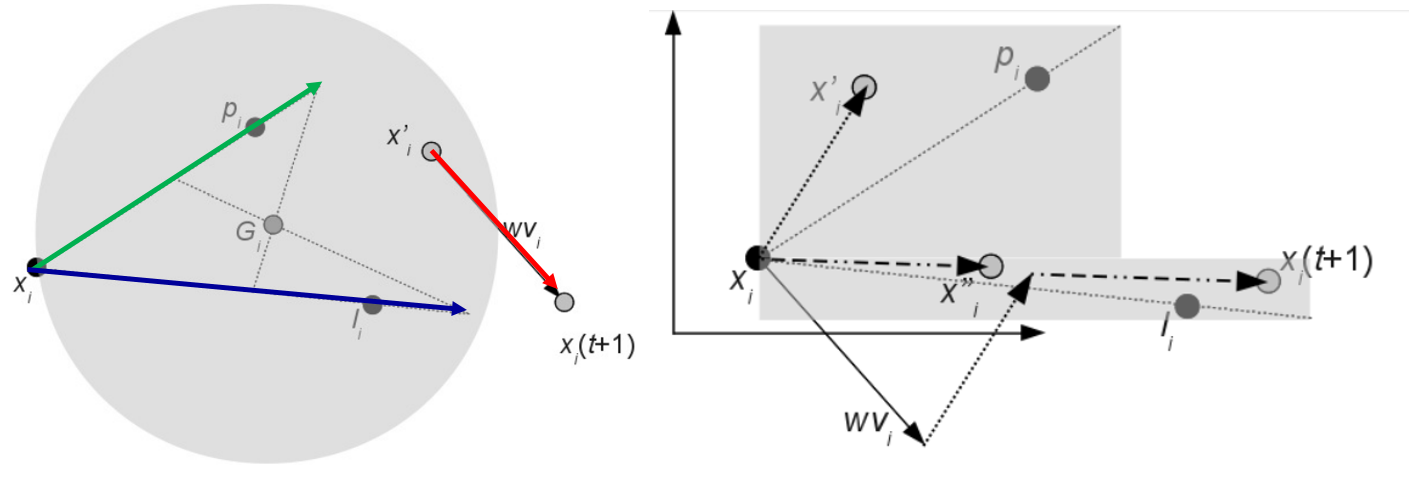
\includegraphics[width=\textwidth]{SPSO_update}
\caption{(a) SPSO 2011. (b) SPSO 2006.}\label{fig:SPSO_update}
\end{figure}

Describe boundary and out-of-bound handling.

\subsection{Random Topology}
Describe random topology and when to update topology.
The information links...  The adaptive random topology described in ~\cite{Clerc:2007:randomTopology} is formally equivalent to "Stocastic Star".



The pseudo code defined in~\cite{Zambrano:2013:SPSO2011}.
The pseudo code is given in Algorithm~\ref{algo:SPSO2011}.



\begin{algorithm}%[t!]
\caption{Standard PSO 2011}\label{algo:SPSO2011}

$\boldsymbol{X}_{n}$: solution of the $n^{th}$ iteration, $\sigma_n$: step size of the $n^{th}$ iteration, \\
$N(\boldsymbol{0}, \boldsymbol{I})$: multivariant normal distribution with mean vector $\boldsymbol{0}$ \\ 
and identical covariance matrix $\boldsymbol{I}$.

\BlankLine
\SetKwInOut{Input}{input} \SetKwInOut{Output}{output}
\Input{ $f$: evaluation function }
\Output{ $X_{n+1}$: best solution }

\BlankLine
Initialize $\boldsymbol{X}_0, \sigma_0$ \\
\While{ termination criterion not met } {

    $\widetilde{\boldsymbol{X}}_n = \boldsymbol{X}_n + \sigma_n N(\boldsymbol{0}, \boldsymbol{I})$  \\

    \eIf{ $f(\widetilde{\boldsymbol{X}}_n) \leq f(\boldsymbol{X}_n) $}{
        $\boldsymbol{X}_{n+1} = \widetilde{\boldsymbol{X}}_n$ \\
        $\sigma_{n+1} = 1.5 \sigma_n$
    }{
        $\boldsymbol{X}_{n+1} = \boldsymbol{X}_n$ \\
        $\sigma_{n+1} = 1.5^{-1/4}\sigma_n$
    }
}

\Return $\boldsymbol{X}_{n+1}$

\end{algorithm}




\section{Ant Colony Optimization for Continuous Domain}

Ant Colony optimization (ACO) is first proposed by Dorigo~\cite{Dorigo:1999:ACO} to solve combinatorial optimization problems, including scheduling, routing, and timetabling.
These problems aim to find optimal \textit{combinations} or \textit{permutations} of finit sets of available components.
Inspired by the foraging behavior of natural ants, ACO mimics the pheromone deposition of ants along the trail to a food source.
The deposited pheromone, which indicates the quantity and quality of the food, creates an indirect communication among ants and enables them to find the shortest paths.
The pseudo code of ACO is given in Algorithm~\ref{algo:ACO}.
Two major procedures: \textit{solution construction} and \textit{phermone update}, are detailed in the following paragraph.


Consider a search space $\boldsymbol{S}$ defined over a finit set of all possible \textit{solution components}, denoted by $\boldsymbol{C}$.
Each solution component, denoted by $c_{ij}$, is a decision variable $X_i$ instantiated with value $v^{j}_{i} \in \boldsymbol{D}_i = \{ v^{1}_{i}, ..., v^{|\boldsymbol{D}_i|}_{i}\}$.
To construct a new solution, an artificial ants starts with an empty partial solution $s^{p} = \emptyset$.
During each construction step, the partial solution $s^{p}$ is extended with a feasible solution from the set $N(s^{p}) \in \boldsymbol{C} \setminus s^{p}$.
The probabilistic pheromone model adopted for selecting a feasible solution from $N(s^{p})$ can be defined as follows:

\begin{equation}
p(c_{ij}|s^p) = \frac{\tau^{\alpha}_{ij} \cdot \eta(c_{ij})^{\beta}} 
                     {\sum_{c_{i\ell}\in N(s^{p})} \tau^{\alpha}_{i\ell} \cdot \eta(c_{i\ell})^{\beta} },  \forall c_{ij} \in N(s^{p}),
\end{equation}
where $\tau_{ij}$ is the pheromone value associated with component $c_{ij}$, and $\eta(\cdot)$ is a weighting function. 
% that assigns at each construction step a heuristic value to each feasible solution component $c_{ij} \in N(s^{p})$.
$\alpha$ and $\beta$ are positive parameters which determine the relation between phermone and heuristic information.

The pheromone update


Over the years, multiple approaches of extending the ACO on continous domain have been given.
One of the most successful version is ACO$_{R}$, proposed by Socha and Dorigo in 2008~\cite{Socha:2008:ACOR}.
It extends ACO to the continuous domain without making any major conceptual change to its structure.
The fundamental idea underlying ACO$_{R}$ is the shift from using a discrete probability distribution to using a continuous one, demonstrated in Figure~\ref{fig:ACOR_distribution}. 

A enhanced Gaussian kernel PDF as shown in Figure~\ref{fig:ACOR_gaussianKernel}.

\begin{figure}
\centering
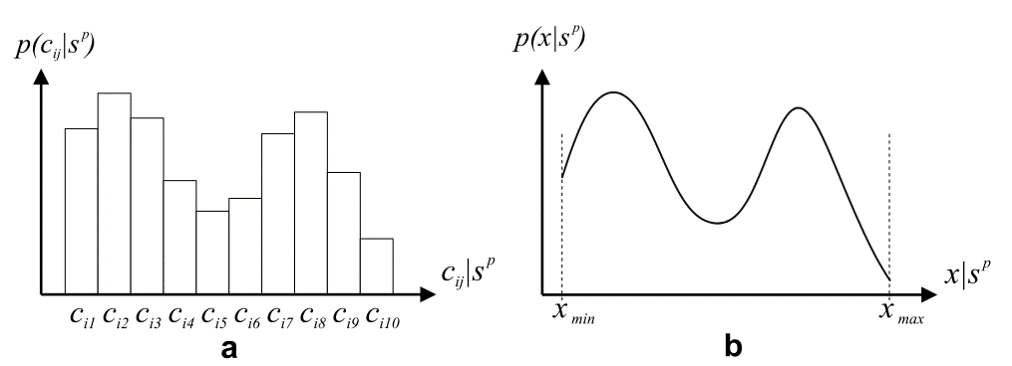
\includegraphics[width=\textwidth]{ACOR_distribution}
\caption{(a) Discrete probability distribution $p(c_{ij}|s^{p})$. (b) Continuous probability density function $p(x|s^{p})$}\label{fig:ACOR_distribution}
\end{figure}

\begin{figure}
\centering
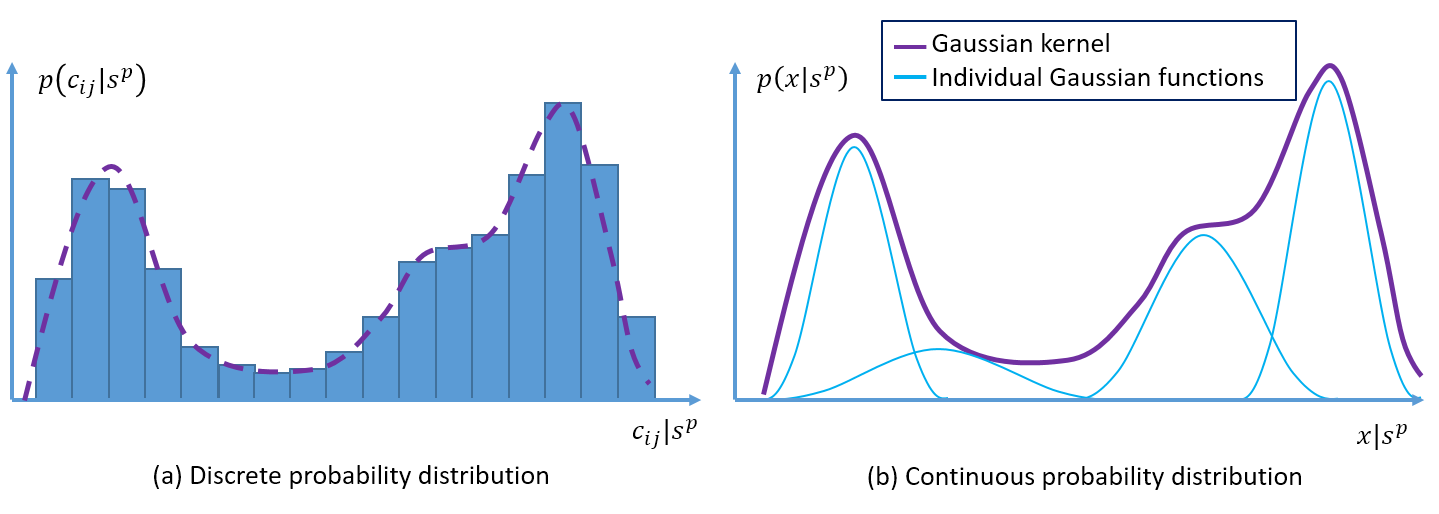
\includegraphics[width=\textwidth]{ACOR_gaussianKernel}
\caption{(a) Discrete probability distribution $p(c_{ij}|s^{p})$. (b) Continuous probability density function $p(x|s^{p})$}\label{fig:ACOR_gaussianKernel}
\end{figure}

\begin{algorithm}%[t!]
\caption{Ant Colony Optimization metaheuristic}\label{algo:ACO}
\While{ termination criterion not met } {

    schedule activities \\
    solution contruction by ants(); \\
    phermone update(); \\
    daemon actions(); \\
}
\end{algorithm}



